En la presente sección, se implementarán cuatro filtros de segundo orden según las siguientes especificaciones:

\begin{table}[H]
    \centering
    \begin{tabular}{|c|c|c|c|}
    \hline
    \rowcolor[HTML]{C0C0C0} 
    Tipo de Filtro & $f_p[Hz]$ & $f_a[Hz]$ & $f_c[Hz]$ \\ \hline
    Low-Pass       & 5000   & 17500  & -      \\ \hline
    High-Pass      & 21000   & 6000   & -      \\ \hline
    Band-Pass      & -      & -      & 10000  \\ \hline
    Band-Rejection & -      & -      & 6000   \\ \hline
    \end{tabular}
    \end{table}

En cada caso se espera:

\begin{itemize}
	\item Ganancia mayor a -3 dB cuando $f < f_p$ o $f > f_p$ 
	\item Ganancia menor a -10 dB cuando $f > f_a$ o $f < f_a$
	\item Ganancia nunca superior a 0 dB
	\item Ganancia unitaria en continua ($f \to \infty$)
\end{itemize}

Cada circuito será empleado implementando una resistencia $R$, una inductancia $L$ y un capacitor $C$. Pero para la
inductancia $L$, ésta será reemplazada por componentes que unidos presenten un comportamiento similar a ella, en este caso
un Gyrator.

\subsection{Filtro Pasa-Bajos (Low-Pass)}

En este caso, se procederá a realizar un circuito pasa-bajos de segundo orden clásico, tal que podemos
ver la disposición de elementos en la siguiente figura:

\begin{figure}[H]
    \centering
    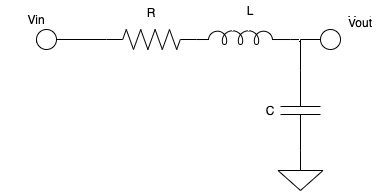
\includegraphics[width=0.6\textwidth]{../Ejercicio2-DiseñoDeFiltros/Imagenes/diagrama-pasa-bajos.png}
    \caption{Circuito Pasa-Bajos de segundo orden}
\end{figure}

Las especificaciones son las siguientes:

\begin{itemize}
	\item E1: Ganancia mayor a -3 dB cuando $f < 5 KHz$ 
	\item E2: Ganancia menor a -10 dB cuando $f > 17.5 KHz $
	\item E3: Ganancia nunca superior a 0 dB
	\item E4: Ganancia unitaria en continua ($f \to \infty$)
\end{itemize}

En el dominio de Laplace podemos ver que la función de transferencia para este circuito está dada por:

$$H(S)=\frac{V_{out}(S)}{V_{in}(S)}=\frac{\frac{1}{SC}}{SL+R+\frac{1}{SC}} \longrightarrow 
H(S)=\frac{1}{S^2LC+SCR+1}$$

De allí podemos observar que $w_0=\frac{1}{\sqrt{LC}}$, $Q=\frac{1}{2\xi}$ y $\xi=\frac{R\sqrt{C}}{2\sqrt{L}}$

Podemos observar que la ganancia nunca deberá superar a 0 dB por ello no se deben presentar sobrepicos en el circuito RLC.
Sabiendo que los sobrepicos se presentarán en casos donde $\xi \leq \frac{1}{\sqrt{2}}$, se tomarán valores que cumplan la relación:

$$\xi > \frac{1}{\sqrt{2}}$$.

Además de ello, para un circuito de segundo orden la pendiente de la recta que se presenta en $H(S)$ es de 
40 $\frac{dB}{dec}$, más precisamente -40 $\frac{dB}{dec}$ en este caso. 

Para establecer una relación y hallar una frecuencia de corte $f_0$ apropiada, tal que se cumplan los requisitos
de la plantilla, estableceremos una diferencia mínima de 10 dB entre $5 KHz$ y $17.5 KHz$, ya que la diferencia establecida por la plantilla
es de por lo menos 7 dB (-3 dB a -10 dB).

Mediante dicha relación, entonces sabiendo que en $\frac{1}{4}$ de década representará una diferencia de 10 dB para dicha pendiente:

$$\frac{1}{4}=\log_{10}(\frac{17.5KHz}{f_0})$$

De esta manera, podremos estimar una $f_0$ tal que se cumpla la plantilla:

$$f_0 = \frac{17.5KHz}{1.7782} = 9.84 KHz$$

Se utilizará una frecuencia un poco menor, $f_0=9 KHz$ ya que con la diferencia establecida de 10 dB, usar una frecuencia menor, no afectará el comportamiento 
esperado según la plantilla.

Entonces por las relaciones expresadas previamente:

$$w_0=\frac{1}{\sqrt{LC}} \longrightarrow 2\pi f_0=\frac{1}{\sqrt{LC}}$$

Luego:

$$\frac{R\sqrt{C}}{2\sqrt{L}} > \frac{1}{\sqrt{2}}$$

Como tenemos varias incógnitas, elegiremos el $C$ a utilizar basándonos en los elementos disponibles, siendo para este caso,
$C=0.1\mu F$. 

Por ello:

$$2\pi 9K=\frac{1}{\sqrt{L0.1 \mu F}} \longrightarrow L = 3.1271 mH$$

Además:

$$\frac{R\sqrt{100n}}{2\sqrt{3.1271m}} > \frac{1}{\sqrt{2}} \longrightarrow R > 249.76 \Omega $$

Es importante notar que a medida que $R$ a nos encontraremos en una situación donde el circuito será
cada vez más sobreamortiguado, por ello buscaremos utilizar un valor de $R$ lo más cercano posible, ya que de otra forma
por la reducción de la pendiente, debido al sobreamortiguamiento podríamos no encontrarnos en los parámetros establecidos en la plantilla. Se utilizó entonces
$R= 330 \Omega$ ya que es el valor más cercano con el que se contaba.

Una vez obtenidos los valores nominales de los elementos, se buscó implementar dicho circuito pero utilizando el gyrator descripto previamente
para reemplazar a la inductancia. Para ello, basándonos 
en las siguientes relaciones:

$$Z=sC_gR_gR_L+R_L$$

$$1 >> sC_gR_L$$

Partiendo de la última expresión, se escogió:

\begin{itemize}
	\item $C_g=0.1 \mu F$
	\item $R_L=10 \Omega$
	\item $R_g=3.3K \Omega$
\end{itemize}

Notar que el valor escogido es tal que $C=C_g$ y $R_L$ es pequeña en comparación a la $R$ del circuito para no generar
un sobreamortiguamiento adicional.

Verificando las relaciones:

$$Z=sC_gR_gR_L+R_L \longrightarrow Z = s3.3m + 10$$

$$1 >> s100n.10 \longrightarrow 1  >> s1\mu$$

Se procedió a simular el comportamiento del circuito RLC equivalente con el gyrator implementado para observar si su comportamiento es el esperado:

%Poner tabla con nuevos valores%

\begin{figure}[H]
    \centering
    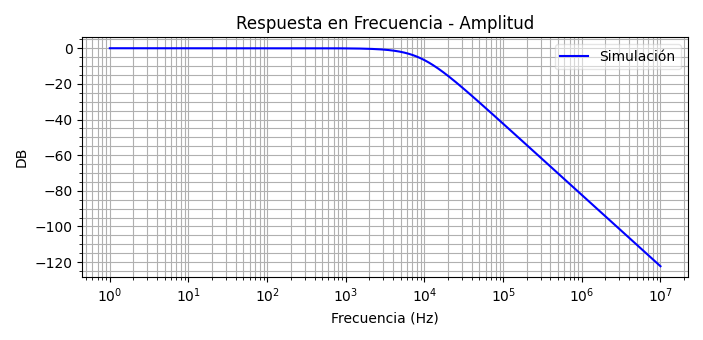
\includegraphics[width=0.6\textwidth]{../Ejercicio2-DiseñoDeFiltros/Imagenes/bode-rlc-pasa-bajos-amplitud.png}
    \caption{Circuito Pasa-Bajos de segundo orden}
\end{figure}

\begin{figure}[H]
    \centering
    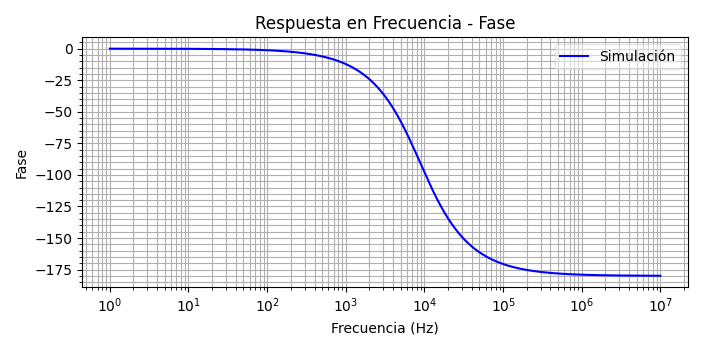
\includegraphics[width=0.6\textwidth]{../Ejercicio2-DiseñoDeFiltros/Imagenes/bode-rlc-pasa-bajos-fase.png}
    \caption{Circuito Pasa-Bajos de segundo orden}
\end{figure}

Se pudo comprobar entonces que para el circuito equivalente con gyrator se cumple lo establecido en la plantilla.
De la simulación se observó que en $f=5.00007 KHz$, la ganancia es de $-1.904 dB$ y en $f=17.503KHz$, es de $-13.25 dB$

Comprobado ello, se realizó la simulación utilizando ahora el amplificador operacional y los elementos pasivos del gyrator obtenidos anteriormente.
Lo obtenido fue lo siguiente:

\begin{figure}[H]
    \centering
    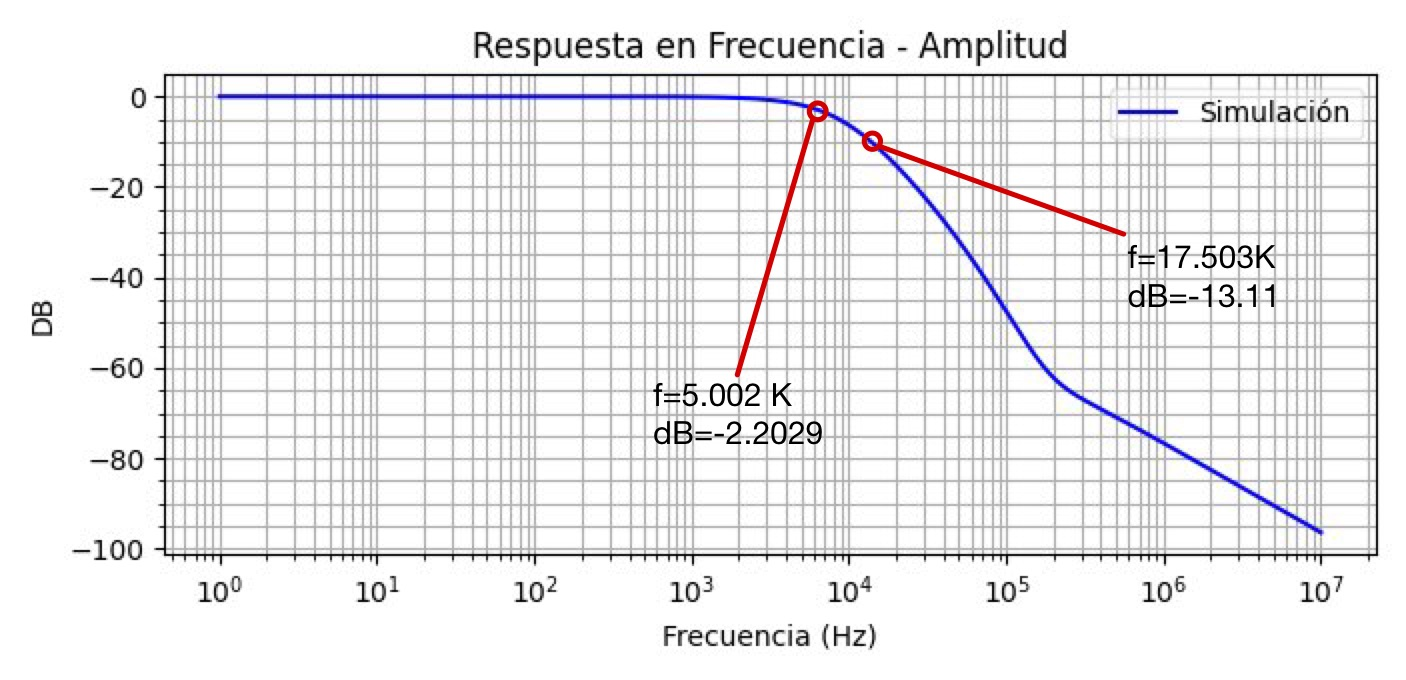
\includegraphics[width=0.6\textwidth]{../Ejercicio2-DiseñoDeFiltros/Imagenes/Pasa-Bajos-Marcado-Opamp.jpg}
    \caption{Circuito Pasa-Bajos de segundo orden}
\end{figure}

\begin{figure}[H]
    \centering
    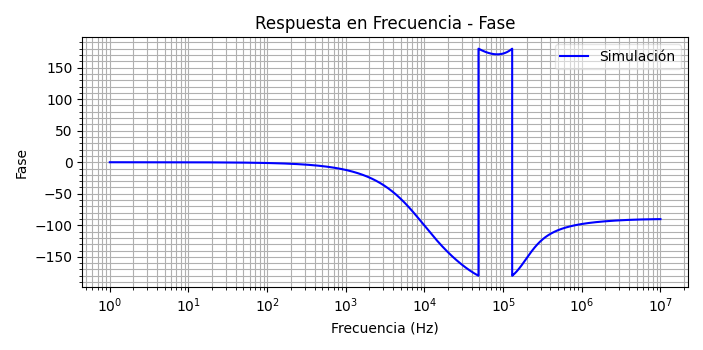
\includegraphics[width=0.6\textwidth]{../Ejercicio2-DiseñoDeFiltros/Imagenes/bode-opamp-pasa-bajos-fase.png}
    \caption{Circuito Pasa-Bajos de segundo orden}
\end{figure}

Se puede comprobar aquí también que la plantilla se sigue cumpliendo obteniendo el filtro pasa-bajos solicitado.

%MEDIR%

\subsection{Filtro Pasa-Altos (High-Pass)}

En este caso, se procederá a realizar un circuito pasa-altos de segundo orden clásico, tal que podemos
ver la disposición de elementos en la siguiente figura:

\begin{figure}[H]
    \centering
    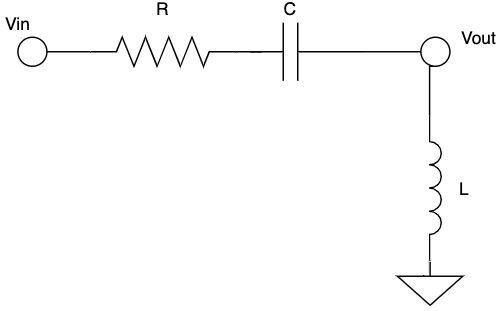
\includegraphics[width=0.6\textwidth]{../Ejercicio2-DiseñoDeFiltros/Imagenes/diagrama-pasa-altos.png}
    \caption{Circuito Pasa-Altos de segundo orden}
\end{figure}

Las especificaciones son las siguientes:

\begin{itemize}
	\item E1: Ganancia mayor a -3 dB cuando $f > 21 KHz$ 
	\item E2: Ganancia menor a -10 dB cuando $f < 6 KHz $
	\item E3: Ganancia nunca superior a 0 dB
	\item E4: Ganancia unitaria en continua ($f \to \infty$)
\end{itemize}

En el dominio de Laplace podemos ver que la función de transferencia para este circuito está dada por:

$$H(S)=\frac{V_{out}(S)}{V_{in}(S)}=\frac{SL}{SL+R+\frac{1}{SC}} \longrightarrow H(S)=\frac{S^{2}LC}{S^2LC+SRC+1}$$

Aquí también podemos observar que $w_0=\frac{1}{\sqrt{LC}}$, $Q=\frac{1}{2\xi}$ y $\xi=\frac{R\sqrt{C}}{2\sqrt{L}}$

Podemos observar que la ganancia nunca deberá superar a 0 dB por ello no se deben presentar sobrepicos en el circuito RLC.
Sabiendo que los sobrepicos se presentarán en casos donde $\xi \leq \frac{1}{\sqrt{2}}$, se tomarán valores que cumplan la relación:

$$\xi > \frac{1}{\sqrt{2}}$$.

Se realizará el mismo análisis que para el circuito pasa-bajos, donde para establecer una relación y hallar una frecuencia de corte $f_0$ apropiada, tal que se cumplan los requisitos
de esta plantilla, estableceremos una diferencia mínima de 10 dB entre $21 KHz$ y $6 KHz$, ya que la diferencia establecida por la plantilla
es de por lo menos 7 dB (-3 dB a -10 dB).

Mediante dicha relación, entonces sabiendo que en $\frac{1}{4}$ de década representará una diferencia de 10 dB para dicha pendiente:

$$\frac{1}{4}=\log_{10}(\frac{17.5KHz}{f_0})$$

De esta manera, podremos estimar una $f_0$ tal que se cumpla la plantilla:

$$f_0 = \frac{21KHz}{1.7782} = 11.80 KHz$$

Se utilizará una frecuencia un poco menor, $f_0=11 KHz$ ya que con la diferencia establecida de 10 dB, usar una frecuencia menor, no afectará el comportamiento 
esperado según la plantilla.

Entonces por las relaciones expresadas previamente:

$$w_0=\frac{1}{\sqrt{LC}} \longrightarrow 2\pi f_0=\frac{1}{\sqrt{LC}}$$

Luego:

$$\frac{R\sqrt{C}}{2\sqrt{L}} > \frac{1}{\sqrt{2}}$$

Como tenemos varias incógnitas, elegiremos el $C$ a utilizar basándonos en los elementos disponibles, siendo para este caso,
$C=0.1\mu F$. 

Por ello:

$$2\pi 11K=\frac{1}{\sqrt{L0.1 \mu F}} \longrightarrow L = 2.0934 mH$$

Además:

$$\frac{R\sqrt{0.1\mu}}{2\sqrt{2.0934m}} > \frac{1}{\sqrt{2}} \longrightarrow R > 204.58 \Omega $$

Es importante notar que a medida que $R$ a nos encontraremos en una situación donde el circuito será
cada vez más sobreamortiguado, por ello buscaremos utilizar un valor de $R$ lo más cercano posible, ya que de otra forma
por la reducción de la pendiente, debido al sobreamortiguamiento podríamos no encontrarnos en los parámetros establecidos en la plantilla. Se utilizó entonces
$R= 220 \Omega$ ya que es el valor más cercano con el que se contaba.

Una vez obtenidos los valores nominales de los elementos, se buscó implementar dicho circuito pero utilizando el gyrator descripto previamente
para reemplazar a la inductancia. Para ello, basándonos 
en las siguientes relaciones:

$$Z=sC_gR_gR_L+R_L$$

$$1 >> sC_gR_L$$

Partiendo de la última expresión, se escogió:

\begin{itemize}
	\item $C_g=0.1 \mu F$
	\item $R_L=10 \Omega$
	\item $R_g=2.2K \Omega$
\end{itemize}

Notar que el valor escogido es tal que $C=C_g$ y $R_L$ es pequeña en comparación a la $R$ del circuito para no generar
un sobreamortiguamiento adicional.

Verificando las relaciones:

$$Z=sC_gR_gR_L+R_L \longrightarrow Z = s2.2m + 10$$

$$1 >> s100n.10 \longrightarrow 1  >> s1\mu$$

Se procedió a simular el comportamiento del circuito RLC equivalente con el gyrator implementado para observar si su comportamiento es el esperado:

%Poner tabla con nuevos valores%

\subsection{Filtro Pasa-Banda (Band-Pass)}
\subsection{Filtro Rechaza-Banda (Band-Rejection)}

1. Diseñar una función transferencia que cumpla con las especificaciones.
2. Diseñar un circuito que implemente la función transferencia utilizando un Gyrator. Justificar adecuadamente la elección de todos sus componentes y redactar una introducción teórica al tema.
3. Determinar rangos de operación en zona lineal. Se espera adecuada profundidad en este análisis.
4. Contrastar el diseño del circuito con las simulaciones correspondientes.
5. Implementar el circuito y comprobar su funcionamiento con las mediciones correspondientes.
6. Analizar el comportamiento del sistema en altas frecuencias.
7. Diseñar un PCB que contenga todos los circuitos pedidos (en el mismo PCB). A su vez, puede utilizarse un
sólo IC en la implementación pedida.

\subsection{Utilización de un Gyrator en los filtros}

En los circuitos descriptos previamente, se reemplazará la inductancia $L$, por un equivalente utilizando
un gyrator. 

\subsubsection{Introducción a Gyrators}

Un Gyrator o girador es considerado un elemento pasivo adicional a los ya conocidos y analizados. Una de sus funcionalidades es ser empleado como un inductor. 
El motivo de reemplazar a un inductor real se encuentra en fines prácticos, ya que al utilizar éste en lugar de una inductancia, se pueden reducir tanto el tamaño de un circuito
como el costo del mismo. 

Además, una inductancia tiene asociada una resistencia. El cable que se utiliza para elaborarlos, tiene dicha resistencia asociada. 
Por otro lado, se pueden obtener capacitores de alta calidad y con un girador, obtener inductores de alta calidad.

Entonces un gyrator puede reemplazar a una inductancia con una combinación de amplificador operacional, una resistencia y un capacitor.
Para lograr ello, podemos definir también al gyrator como un inversor de las características corriente voltaje de un componente eléctrico.

El símbolo circuital utilizado para el gyrator es el siguiente:

\begin{figure}[H]
    \centering
    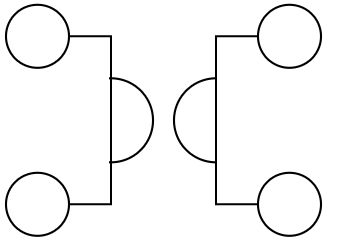
\includegraphics[width=0.3\textwidth]{../Ejercicio2-DiseñoDeFiltros/Imagenes/diagrama-basico-gyrator.png}
    \caption{Símbolo circuital del Gyrator}
\end{figure}

\subsubsection{Implementación real de un Gyrator}

Físicamente hay distintas formas de implementar un Gyrator, pero en nuestro caso, lo implementaremos con un solo elemento activo representado
por un amplificador operacional aunque se han visto en la cátedra formas de implementarlo con dos amplificadores, con el fin de simplificar las mediciones
y armado de circuito se analizará el caso con un solo amplificador.

En el siguiente diagrama se puede ver dicha implementación observando el Gyrator a la izquierda y su equivalente a la derecha:

\begin{figure}[H]
    \centering
    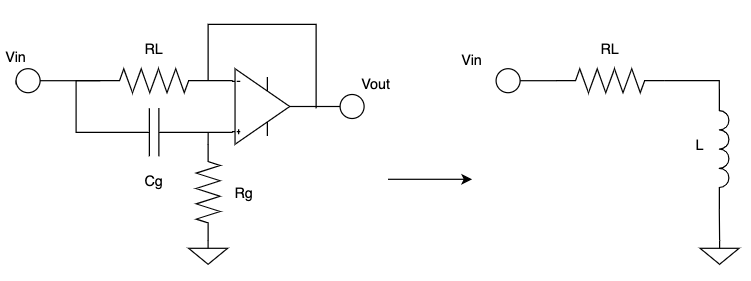
\includegraphics[width=0.6\textwidth]{../Ejercicio2-DiseñoDeFiltros/Imagenes/diagrama-gyrator-inductor.png}
    \caption{Equivalente circuital entre Gyrator e Inductor}
\end{figure}

En la próxima sección se verá que este equivalente no es válido para todo el rango de frecuencias.

\subsubsection{Análisis de $Z_{in}$}

Para describir el comportamiento del circuito como un inductor es importante 
analizar la impedancia de entrada de dicho circuito tal que $Z_{in}=\frac{V_{in}}{I_{in}}$. 
Para ello, utilizaremos el siguiente diagrama circuital:

\begin{figure}[H]
    \centering
    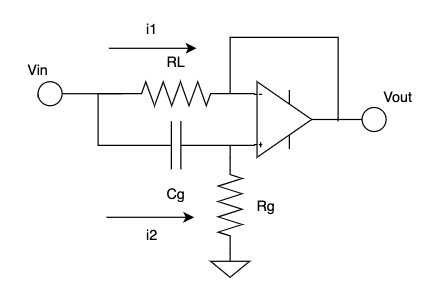
\includegraphics[width=0.4\textwidth]{../Ejercicio2-DiseñoDeFiltros/Imagenes/diagrama-gyrator-corrientes.png}
    \caption{Equivalente circuital entre Gyrator e Inductor}
\end{figure}

Se puede observar del gráfico que:

$$V_{out}=V^-$$

Por ello:

$$V_{out}=A_{vol}(V^+-V^-) \longrightarrow V^-=A_{vol}(V^+-V^-) 
\longrightarrow V^-= V^+ \frac{A_{vol}}{1+A_{vol}}$$

Luego podemos ver utilizando un divisor de tensión que:

$$V^+= V_{in}\frac{R_g}{R_g+\frac{1}{sC_g}}$$

Además obsevamos que:

$$I_{in}=i_1+i_2$$

Como no ingresa corriente al amplificador operacional:

$$i_1=\frac{V_{in}-V^-}{R_L}$$
$$i_2=\frac{V^+}{R_g}$$

Entonces:

$$I_{in}=\frac{V_{in}-V^-}{R_L}+\frac{V^+}{R_g} \longrightarrow 
I_{in}=V_{in}(\frac{R_g+\frac{1}{sC_g}+R_L-R_g\frac{A_{vol}}{1+A_{vol}}}{R_L(R_g+\frac{1}{sC_g})})$$

Finalmente:

$$Z_{in}=\frac{V_{in}}{I_{in}}=\frac{V_{in}}{V_{in}(\frac{R_g+\frac{1}{sC_g}+R_L-R_g\frac{A_{vol}}{1+A_{vol}}}{R_L(R_g+\frac{1}{sC_g})})}$$

$$Z_{in}=\frac{R_L(R_g+\frac{1}{sC_g})}{R_g+\frac{1}{sC_g}+R_L-R_g\frac{A_{vol}}{1+A_{vol}}}$$

Si ahora multiplicamos por el factor $sC_g$ en numerador y denominador:

$$Z_{in}=\frac{R_L(sC_gR_g+1)}{sC_g(R_g+R_L-R_g\frac{A_{vol}}{1+A_{vol}})+1}$$

Como $A_{vol}=\frac{A_0}{1+\frac{s}{w_p}}$, el factor $\frac{A_{vol}}{1+A_{vol}}$ cambia su comportamiento
según la frecuencia de trabajo:

$$\frac{A_{vol}}{1+A_{vol}}=\frac{\frac{A_0}{1+\frac{s}{w_p}}}{1+\frac{A_0}{1+\frac{s}{w_p}}}=
\frac{A_0}{A_0+1+\frac{s}{w_p}}=\frac{1}{1+\frac{1}{A_0}+\frac{s}{A_0w_p}}$$

Notemos que $GBP$ o Gain Bandwidth Product es equivalente a $A_0w_p$, y $A_0$ tiene un valor alto, por ello:

$$\frac{1}{1+\frac{s}{GBP}}$$

Entonces, siempre que $\frac{s}{GBP} >> 1$ , podremos aproximar dicha expresión:

$$\frac{1}{1+\frac{s}{GBP}} \approx 1$$

Siendo:

$$Z_{in}=\frac{R_L(sC_gR_g+1)}{sC_gR_L+1}$$

Tomaremos dicha relación cuando $\frac{s}{GBP} \geq 10$, o equivalente a decir una diferencia de un orden de magnitud.

Caso contrario, nuestro impedancia no podrá aproximarse a un inductor.

Como $Z_{in}=\frac{R_L(sC_gR_g+1)}{sC_gR_L+1}$, para obtener una expresión de la forma de un inductor,
podremos establecer las siguientes relaciones tal que:

$$1 >> sC_gR_L$$

Cumpliendo dicha situación, nuestro inductor usando gyrator estará representado por:

$Z_{in}=R_L(sC_gR_g+1)\longrightarrow Z_{in}=sC_gR_gR_L+R_L$

Donde:

$$L=C_gR_gR_L$$

Como nota final de este comportamiento es importante ver que la relación $1 >> sC_gR_L$, se cumplirá a bajas frecuencias,
mayores o menores dependiendo de los componentes elegidos. Además de ello, el Gyrator para ser empleado como inductor deberá estar
siempre referenciado a tierra. Nuestro equivalente quedará representado por:

\begin{figure}[H]
    \centering
    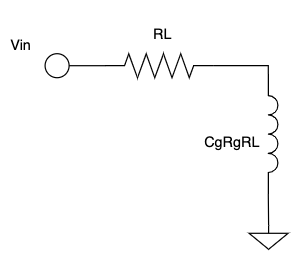
\includegraphics[width=0.3\textwidth]{../Ejercicio2-DiseñoDeFiltros/Imagenes/equivalente-inductor.png}
    \caption{Equivalente de Inductor utilizando un Gyrator}
\end{figure}


